% 母子相似 例1：p=4, q=9, h=6, c=13, b=2√13, a=3√13
\documentclass[tikz,border=4pt]{standalone}
\usepackage{ctex}
\usepackage{amsmath}
\usetikzlibrary{calc}
\begin{document}
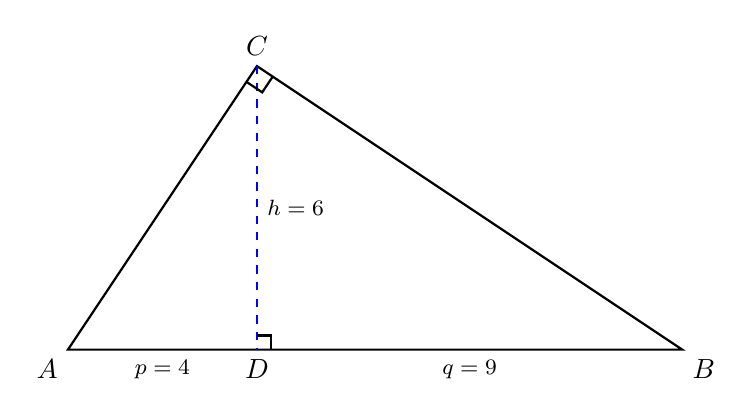
\begin{tikzpicture}[scale=0.6, thick]
  % AB=13. AD=4 -> D=(4,0). h=6, C=(4,6).
  \coordinate (A) at (0,0);
  \coordinate (B) at (13,0);
  \coordinate (D) at (4,0);
  \coordinate (C) at (4,6);
  \draw (A)--(B)--(C)--cycle;
  \draw[blue, dashed] (C)--(D);
  % 直角 C
  % AC 方向 atan2(6,4), CB 方向 atan2(-6,9), 它们应垂直
  \draw ($(C)+({0.4*cos(atan2(-6,9))},{0.4*sin(atan2(-6,9))})$)
        -- ($(C)+({0.4*cos(atan2(-6,9))+0.4*cos(180+atan2(6,4))},{0.4*sin(atan2(-6,9))+0.4*sin(180+atan2(6,4))})$)
        -- ($(C)+({0.4*cos(180+atan2(6,4))},{0.4*sin(180+atan2(6,4))})$);
  % 直角 D
  \draw ($(D)+(0.3,0)$) -- ($(D)+(0.3,0.3)$) -- ($(D)+(0,0.3)$);
  \node[below left] at (A) {$A$};
  \node[below right] at (B) {$B$};
  \node[above] at (C) {$C$};
  \node[below] at (D) {$D$};
  \node[below] at ($(A)!0.5!(D)$) {\footnotesize $p=4$};
  \node[below] at ($(D)!0.5!(B)$) {\footnotesize $q=9$};
  \node[right] at ($(C)!0.5!(D)$) {\footnotesize $h=6$};
\end{tikzpicture}
\end{document}
